% Options for packages loaded elsewhere
\PassOptionsToPackage{unicode}{hyperref}
\PassOptionsToPackage{hyphens}{url}
%
\documentclass[
]{article}
\usepackage{amsmath,amssymb}
\usepackage{lmodern}
\usepackage{ifxetex,ifluatex}
\ifnum 0\ifxetex 1\fi\ifluatex 1\fi=0 % if pdftex
  \usepackage[T1]{fontenc}
  \usepackage[utf8]{inputenc}
  \usepackage{textcomp} % provide euro and other symbols
\else % if luatex or xetex
  \usepackage{unicode-math}
  \defaultfontfeatures{Scale=MatchLowercase}
  \defaultfontfeatures[\rmfamily]{Ligatures=TeX,Scale=1}
\fi
% Use upquote if available, for straight quotes in verbatim environments
\IfFileExists{upquote.sty}{\usepackage{upquote}}{}
\IfFileExists{microtype.sty}{% use microtype if available
  \usepackage[]{microtype}
  \UseMicrotypeSet[protrusion]{basicmath} % disable protrusion for tt fonts
}{}
\makeatletter
\@ifundefined{KOMAClassName}{% if non-KOMA class
  \IfFileExists{parskip.sty}{%
    \usepackage{parskip}
  }{% else
    \setlength{\parindent}{0pt}
    \setlength{\parskip}{6pt plus 2pt minus 1pt}}
}{% if KOMA class
  \KOMAoptions{parskip=half}}
\makeatother
\usepackage{xcolor}
\IfFileExists{xurl.sty}{\usepackage{xurl}}{} % add URL line breaks if available
\IfFileExists{bookmark.sty}{\usepackage{bookmark}}{\usepackage{hyperref}}
\hypersetup{
  pdftitle={ST 563 Final Project - Bike Sharing Data},
  pdfauthor={Peter Lung, David Shaw, Yijia Cai},
  hidelinks,
  pdfcreator={LaTeX via pandoc}}
\urlstyle{same} % disable monospaced font for URLs
\usepackage[margin=1in]{geometry}
\usepackage{color}
\usepackage{fancyvrb}
\newcommand{\VerbBar}{|}
\newcommand{\VERB}{\Verb[commandchars=\\\{\}]}
\DefineVerbatimEnvironment{Highlighting}{Verbatim}{commandchars=\\\{\}}
% Add ',fontsize=\small' for more characters per line
\usepackage{framed}
\definecolor{shadecolor}{RGB}{248,248,248}
\newenvironment{Shaded}{\begin{snugshade}}{\end{snugshade}}
\newcommand{\AlertTok}[1]{\textcolor[rgb]{0.94,0.16,0.16}{#1}}
\newcommand{\AnnotationTok}[1]{\textcolor[rgb]{0.56,0.35,0.01}{\textbf{\textit{#1}}}}
\newcommand{\AttributeTok}[1]{\textcolor[rgb]{0.77,0.63,0.00}{#1}}
\newcommand{\BaseNTok}[1]{\textcolor[rgb]{0.00,0.00,0.81}{#1}}
\newcommand{\BuiltInTok}[1]{#1}
\newcommand{\CharTok}[1]{\textcolor[rgb]{0.31,0.60,0.02}{#1}}
\newcommand{\CommentTok}[1]{\textcolor[rgb]{0.56,0.35,0.01}{\textit{#1}}}
\newcommand{\CommentVarTok}[1]{\textcolor[rgb]{0.56,0.35,0.01}{\textbf{\textit{#1}}}}
\newcommand{\ConstantTok}[1]{\textcolor[rgb]{0.00,0.00,0.00}{#1}}
\newcommand{\ControlFlowTok}[1]{\textcolor[rgb]{0.13,0.29,0.53}{\textbf{#1}}}
\newcommand{\DataTypeTok}[1]{\textcolor[rgb]{0.13,0.29,0.53}{#1}}
\newcommand{\DecValTok}[1]{\textcolor[rgb]{0.00,0.00,0.81}{#1}}
\newcommand{\DocumentationTok}[1]{\textcolor[rgb]{0.56,0.35,0.01}{\textbf{\textit{#1}}}}
\newcommand{\ErrorTok}[1]{\textcolor[rgb]{0.64,0.00,0.00}{\textbf{#1}}}
\newcommand{\ExtensionTok}[1]{#1}
\newcommand{\FloatTok}[1]{\textcolor[rgb]{0.00,0.00,0.81}{#1}}
\newcommand{\FunctionTok}[1]{\textcolor[rgb]{0.00,0.00,0.00}{#1}}
\newcommand{\ImportTok}[1]{#1}
\newcommand{\InformationTok}[1]{\textcolor[rgb]{0.56,0.35,0.01}{\textbf{\textit{#1}}}}
\newcommand{\KeywordTok}[1]{\textcolor[rgb]{0.13,0.29,0.53}{\textbf{#1}}}
\newcommand{\NormalTok}[1]{#1}
\newcommand{\OperatorTok}[1]{\textcolor[rgb]{0.81,0.36,0.00}{\textbf{#1}}}
\newcommand{\OtherTok}[1]{\textcolor[rgb]{0.56,0.35,0.01}{#1}}
\newcommand{\PreprocessorTok}[1]{\textcolor[rgb]{0.56,0.35,0.01}{\textit{#1}}}
\newcommand{\RegionMarkerTok}[1]{#1}
\newcommand{\SpecialCharTok}[1]{\textcolor[rgb]{0.00,0.00,0.00}{#1}}
\newcommand{\SpecialStringTok}[1]{\textcolor[rgb]{0.31,0.60,0.02}{#1}}
\newcommand{\StringTok}[1]{\textcolor[rgb]{0.31,0.60,0.02}{#1}}
\newcommand{\VariableTok}[1]{\textcolor[rgb]{0.00,0.00,0.00}{#1}}
\newcommand{\VerbatimStringTok}[1]{\textcolor[rgb]{0.31,0.60,0.02}{#1}}
\newcommand{\WarningTok}[1]{\textcolor[rgb]{0.56,0.35,0.01}{\textbf{\textit{#1}}}}
\usepackage{graphicx}
\makeatletter
\def\maxwidth{\ifdim\Gin@nat@width>\linewidth\linewidth\else\Gin@nat@width\fi}
\def\maxheight{\ifdim\Gin@nat@height>\textheight\textheight\else\Gin@nat@height\fi}
\makeatother
% Scale images if necessary, so that they will not overflow the page
% margins by default, and it is still possible to overwrite the defaults
% using explicit options in \includegraphics[width, height, ...]{}
\setkeys{Gin}{width=\maxwidth,height=\maxheight,keepaspectratio}
% Set default figure placement to htbp
\makeatletter
\def\fps@figure{htbp}
\makeatother
\setlength{\emergencystretch}{3em} % prevent overfull lines
\providecommand{\tightlist}{%
  \setlength{\itemsep}{0pt}\setlength{\parskip}{0pt}}
\setcounter{secnumdepth}{-\maxdimen} % remove section numbering
\usepackage{booktabs}
\usepackage{longtable}
\usepackage{array}
\usepackage{multirow}
\usepackage{wrapfig}
\usepackage{float}
\usepackage{colortbl}
\usepackage{pdflscape}
\usepackage{tabu}
\usepackage{threeparttable}
\usepackage{threeparttablex}
\usepackage[normalem]{ulem}
\usepackage{makecell}
\usepackage{xcolor}
\ifluatex
  \usepackage{selnolig}  % disable illegal ligatures
\fi

\title{ST 563 Final Project - Bike Sharing Data}
\usepackage{etoolbox}
\makeatletter
\providecommand{\subtitle}[1]{% add subtitle to \maketitle
  \apptocmd{\@title}{\par {\large #1 \par}}{}{}
}
\makeatother
\subtitle{Team \#1}
\author{Peter Lung, David Shaw, Yijia Cai}
\date{11/4/2021}

\begin{document}
\maketitle

\newpage

\hypertarget{introduction}{%
\subsection{Introduction}\label{introduction}}

For our project, we are analyzing the bike sharing dataset from the UCI
Machine Learning database. The data is the number of daily bike rentals
(registered plus ``casual'') over a two year period. Predictors for this
model include variables pertaining to seasonality and weather.

The following is the description of the data from UCI's ML database:

\emph{Bike sharing systems are new generation of traditional bike
rentals where whole process from membership, rental and return back has
become automatic. Through these systems, user is able to easily rent a
bike from a particular position and return back at another position.
Currently, there are about over 500 bike-sharing programs around the
world which is composed of over 500 thousands bicycles. Today, there
exists great interest in these systems due to their important role in
traffic, environmental and health issues.}

\emph{Apart from interesting real world applications of bike sharing
systems, the characteristics of data being generated by these systems
make them attractive for the research. Opposed to other transport
services such as bus or subway, the duration of travel, departure and
arrival position is explicitly recorded in these systems. This feature
turns bike sharing system into a virtual sensor network that can be used
for sensing mobility in the city. Hence, it is expected that most of
important events in the city could be detected via monitoring these
data.}

The response variable from this dataset is \emph{cnt} which is the total
daily count of bike renters. Two other response variables are present in
the dataset: \emph{registered} and \emph{casual}. The response we have
chosen is \emph{cnt}, which is the sum of the other two.

Our interest is twofold:

\begin{enumerate}
\def\labelenumi{(\arabic{enumi})}
\item
  Find the best function of the variable set for predicting the response
\item
  Evaluate several candidate modeling types for variable selection and
  data reduction
\end{enumerate}

The predictor variables all pertain to either weather conditions or
seasonal effects, some of which can be highly collinear. That makes this
data a great set for testing variable selection methods including
forward, backward, best subsets, lasso and ridge. It also makes this
data a great candidate for testing data reduction methods such as
principal components analysis.

We are also interested in testing which variables have nonlinear effects
and modeling them with splines. In all tests, we will evaluate the
models with cross validation and test each model's predictive power with
a consistent holdout sample.

\hypertarget{methods}{%
\subsection{Methods}\label{methods}}

This section will detail the methodologies and evaluations used for each
type of model tested.

\hypertarget{exploratory-data-analysis}{%
\subsubsection{Exploratory Data
Analysis}\label{exploratory-data-analysis}}

\begin{Shaded}
\begin{Highlighting}[]
\CommentTok{\#Required: install remotes package }
\CommentTok{\#install.packages("remotes")}
\CommentTok{\# install corrmorant from the github repository}
\CommentTok{\#remotes::install\_github("r{-}link/corrmorant")}

\CommentTok{\#Check out the dataset}
\FunctionTok{head}\NormalTok{(day)}
\end{Highlighting}
\end{Shaded}

\begin{verbatim}
## # A tibble: 6 x 14
##   instant dteday     season    yr  mnth holiday weekday workingday weathersit
##     <dbl> <date>      <dbl> <dbl> <dbl>   <dbl>   <dbl>      <dbl>      <dbl>
## 1       1 2011-01-01      1     0     1       0       6          0          2
## 2       2 2011-01-02      1     0     1       0       0          0          2
## 3       3 2011-01-03      1     0     1       0       1          1          1
## 4       4 2011-01-04      1     0     1       0       2          1          1
## 5       5 2011-01-05      1     0     1       0       3          1          1
## 6       6 2011-01-06      1     0     1       0       4          1          1
## # ... with 5 more variables: temp <dbl>, atemp <dbl>, hum <dbl>,
## #   windspeed <dbl>, cnt <dbl>
\end{verbatim}

\begin{Shaded}
\begin{Highlighting}[]
\FunctionTok{dim}\NormalTok{(day)}
\end{Highlighting}
\end{Shaded}

\begin{verbatim}
## [1] 731  14
\end{verbatim}

\begin{Shaded}
\begin{Highlighting}[]
\CommentTok{\#Mapping the amount of cnt based on 4 seasons, coloring points by weather conditions}
\FunctionTok{ggplot}\NormalTok{(day,}\FunctionTok{aes}\NormalTok{(cnt,season,}\AttributeTok{color=}\NormalTok{weathersit)) }\SpecialCharTok{+} \FunctionTok{geom\_point}\NormalTok{()}
\end{Highlighting}
\end{Shaded}

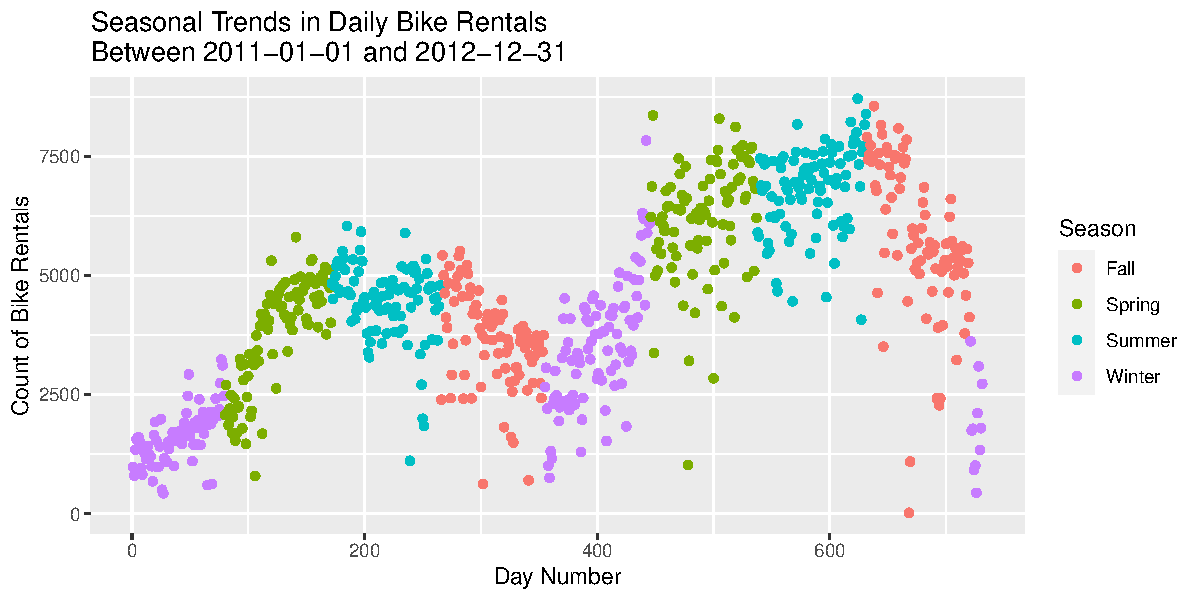
\includegraphics{ST-563-Final-Project_files/figure-latex/unnamed-chunk-1-1.pdf}

\begin{Shaded}
\begin{Highlighting}[]
\FunctionTok{library}\NormalTok{(corrmorant)}
\FunctionTok{ggcorrm}\NormalTok{(}\AttributeTok{data =}\NormalTok{ day[,}\FunctionTok{c}\NormalTok{(}\DecValTok{3}\NormalTok{, }\DecValTok{7}\SpecialCharTok{:}\DecValTok{14}\NormalTok{)]) }\SpecialCharTok{+}
  \FunctionTok{lotri}\NormalTok{(}\FunctionTok{geom\_point}\NormalTok{(}\AttributeTok{alpha =} \FloatTok{0.5}\NormalTok{)) }\SpecialCharTok{+}
  \FunctionTok{utri\_corrtext}\NormalTok{() }\SpecialCharTok{+}
  \FunctionTok{dia\_names}\NormalTok{(}\AttributeTok{y\_pos =} \FloatTok{0.15}\NormalTok{, }\AttributeTok{size =} \DecValTok{3}\NormalTok{) }\SpecialCharTok{+}
  \FunctionTok{dia\_density}\NormalTok{(}\AttributeTok{lower =} \FloatTok{0.3}\NormalTok{, }\AttributeTok{fill =} \StringTok{"grey80"}\NormalTok{, }\AttributeTok{color =} \DecValTok{1}\NormalTok{)}
\end{Highlighting}
\end{Shaded}

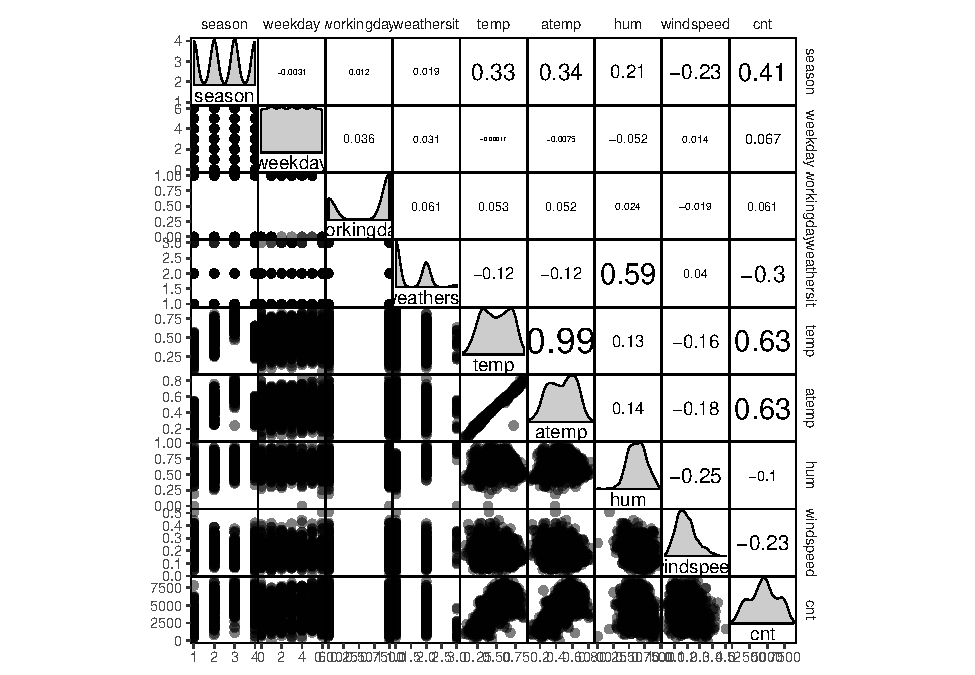
\includegraphics{ST-563-Final-Project_files/figure-latex/unnamed-chunk-1-2.pdf}

Based on the correlation plot, the upper triangle shows the correlation
strength that temp(0.63), atemp(0.63) and Season(0.41) have strong
correlation with the response variable(cnt). At the same time, the lower
triangle scatter plot tells that when weathersit equal to 3 there might
be some correlations there can be analysed.

\hypertarget{lasso-regression}{%
\subsubsection{Lasso Regression}\label{lasso-regression}}

\hypertarget{variable-selection-methods}{%
\paragraph{Variable Selection
Methods}\label{variable-selection-methods}}

\hypertarget{splines-to-capture-nonlinear-effects}{%
\paragraph{Splines to Capture Nonlinear
Effects}\label{splines-to-capture-nonlinear-effects}}

Splines capture nonlinear effects by allowing the model to fit a smooth
linear curve from a set of cubic functions onto the data. The general
form for a cubic spline in a simple linear regression model is:

\[y_i = \beta_0 + \beta_1 x_i + \beta_2 x_i^2 + \beta_3 x_i^3 + \sum_{k = 1}^K \left( \beta_{k + 3} (x_i - t_k)^3 \cdot I_{x_i > t_k} \right) + \varepsilon_i\]

Where the summation represents as series of \(K\) terms that capture
nonlinear effects at different intervals of the predictor variable.

\hypertarget{model-selection}{%
\paragraph{Model Selection}\label{model-selection}}

\hypertarget{ridge-regression}{%
\subsubsection{Ridge Regression}\label{ridge-regression}}

\hypertarget{variable-selection-methods-1}{%
\paragraph{Variable Selection
Methods}\label{variable-selection-methods-1}}

\hypertarget{splines-to-capture-nonlinear-effects-1}{%
\paragraph{Splines to Capture Nonlinear
Effects}\label{splines-to-capture-nonlinear-effects-1}}

\hypertarget{model-selection-1}{%
\paragraph{Model Selection}\label{model-selection-1}}

\hypertarget{principal-components-analysis}{%
\subsubsection{Principal Components
Analysis}\label{principal-components-analysis}}

The third method we utilize for prediction is Principal Components
Regression. PCR is an unsupervised dimension reduction technique which
seeks to draw the maximum variation from each candidate variable into
individual components. In this model, we will attempt to achieve minimum
test error by selecting a subset of the data in the form of the first
\(k\) components.

As with the other models, we will attempt to utilize cubic splines of
the individual components from the training set and use 5 fold cross
validation to do model selection. The principal components will only be
done on continuous variables in the dataset, which include:

\begin{itemize}
\item
  Temperature
\item
  Ambient Temperature
\item
  Humidity
\item
  Wind Speed
\end{itemize}

Seasonal categorical variables will be added to the regression analysis
along with splines of the principal components selected for inclusion.
Certain categorical variables are coded numerically (such as day of the
week and month of the year) so these variables will be modeled with
natural cubic splines. Other variables will be coded as simple dummy
variables in the final regression model.

\hypertarget{pca-and-component-selection}{%
\paragraph{PCA and Component
Selection}\label{pca-and-component-selection}}

\textbf{Move table and plots to appendix!!}

The first step is to perform PCA on the four continuous variables. Each
variable is both scaled and centered in preparation for entering the
principal components procedure. This ensures that each variable has
comparable variability with the others.

Since each variable is standardized, the total variation in the
predictors is simple the number of predictors, which is 4. The following
table displays the proportion of the variance from each of the four
principal components as well as the cumulative variance.

As can be seen in the table, 80\% of the variation in the predictors is
captured in the first two components and nearly all of the variation is
captured in the first three. This is partially a result of the very
strong correlation between temperature and ambient temperature. From
this we can conclude that principal components will be effective at
reducing the dimensionality of the data.

Although the dimensionality of the data is successfully reduced, the
relationship between the components and the response variable determine
the overall quality of the model. The following scatterplots show the
relationship between each component and the response in the training
data:

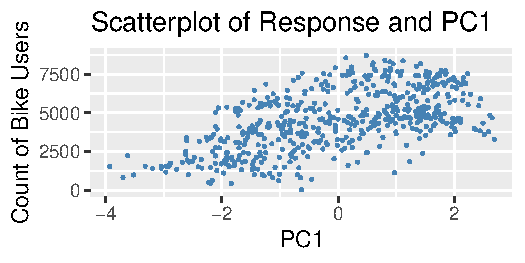
\includegraphics{ST-563-Final-Project_files/figure-latex/PCA_scatter-1.pdf}
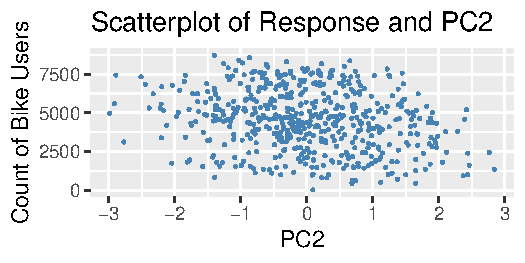
\includegraphics{ST-563-Final-Project_files/figure-latex/PCA_scatter-2.pdf}
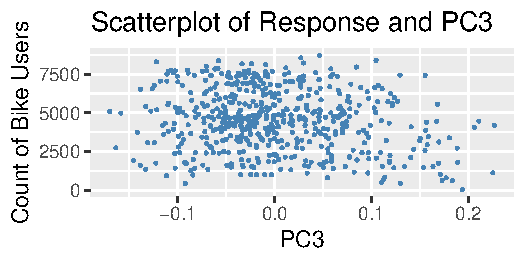
\includegraphics{ST-563-Final-Project_files/figure-latex/PCA_scatter-3.pdf}
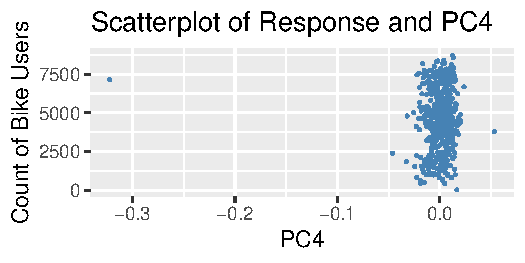
\includegraphics{ST-563-Final-Project_files/figure-latex/PCA_scatter-4.pdf}

The relationships between the individual components and the response are
most pronounced in PC1 and PC2. PC1 looks like it may have a nonlinear
effect on the response being somewhat flat on the low and high parts on
the component and a positive relationship in between. The second
component has what appears to be a negative effect on the response. The
other two components don't appear to have any obvious relationship with
Bike Sharing Counts based on the graph.

\hypertarget{splines-to-capture-nonlinear-effects-of-the-components}{%
\paragraph{Splines to Capture Nonlinear Effects of the
Components}\label{splines-to-capture-nonlinear-effects-of-the-components}}

As in the preceding sections, cubic splines will be used to capture
nonlinear effects of the components. In the case of PCA, the
interpretation of the regression estimates from these splines is
complicated by the fact that components are functions of a series of
variables and not the original variables themselves. As such, there will
be no attempt here to interpret coefficients, but rather to assess fit
and predictive power.

The splines being used are natural cubic splines. The cumulative
variation has suggested that PC4 contains very little of the variation
from the predictors and will be omitted from the model selection
procedure. The graphical analysis has suggested that while PC1 certainly
seems to have nonlinear effects present, it is uncertain whether PC2 or
PC3 have nonlinear effects, or whether they should be included in the
model. As such, they will both be tested for spline effects.

\hypertarget{model-selection-2}{%
\paragraph{Model Selection}\label{model-selection-2}}

The final model is a linear regression model which utilizes cubic
splines for the components PC1 - PC3 as well as day of week and month of
year. Other variables consist of seasonal predictors coded as dummy
variables, including:

\begin{itemize}
\item
  Weather situation
\item
  Holiday
\item
  Year
\end{itemize}

Working day, while present in the dataset, is excluded since it is a
function of the day of the week.

Model selection was performed using 5-fold cross-validation to determine
to optimal degrees of freedom parameter to use for the natural cubic
spline for each component. The degrees of freedom that produced the
smallest cross validation MSE for each variable are included in the
final model selected.

The regression analysis was tested for including three combinations of
the principal components including

\begin{itemize}
\item
  Just PC1
\item
  PC1 and PC2
\item
  PC1, PC2 and PC3
\end{itemize}

All other variables are allowed into the model specification.

\hypertarget{conclusions}{%
\subsection{Conclusions}\label{conclusions}}

\hypertarget{performance-on-the-holdout-dataset}{%
\subsubsection{Performance on the Holdout
Dataset}\label{performance-on-the-holdout-dataset}}

\hypertarget{commentary-on-model-performance}{%
\subsubsection{Commentary on Model
Performance}\label{commentary-on-model-performance}}

\hypertarget{appendix}{%
\subsection{Appendix}\label{appendix}}

\hypertarget{references}{%
\subsection{References}\label{references}}

\end{document}
